\section{Overview of the Quadtree-Adaptive HPS Method}
\label{sec:overview-of-the-quadtree-adaptive-hps-method}

In this section, we provide an overview of the quadtree-adaptive HPS method that is outlined in more detail in \citep{chipman2024fast}. This is to provide context as well as demonstrate where we can implement distributed memory parallelism.

\subsection{Problem Statement and Domain Representation}
\label{sub:problem-statement-and-domain-representation}

The problem we wish to solve is the following variable coefficient elliptic PDE subject to Dirichlet or Neumann boundary conditions:

\begin{align}
    \label{eq:elliptic-pde}
    \nabla \cdot \left( \beta(\textbf{x}) \nabla u(\textbf{x}) \right) + \lambda(\textbf{x}) u(\textbf{x}) &= f(\textbf{x}), \textbf{x} \in \Omega \subset \mathcal{R}^2 \\
    \label{eq:elliptic-pde-bc1}
    u(\textbf{x}) &= g(\textbf{x}), \textbf{x} \in \Gamma_D \subset \Omega \\
    \label{eq:elliptic-pde-bc2}
    \frac{\partial u}{\partial n} \Big|_{\textbf{x}} &= v(\textbf{x}), \textbf{x} \in \Gamma_N \subset \Omega.
\end{align}

The domain $\Omega$ is partitioned into a composite collection of subdomains $\Omega_i$ such that $\Omega = \cup_{i = 1}^{N} \Omega_i$. This is displayed in \reffig{fig:adaptive_mesh}. These subdomains are organized into a {\em leaf-indexed quadtree}
\begin{align}
    \mathcal{Q}_L = \{\Omega_i | i = 1, \dots, N_L\},
\end{align}
where $N_L$ is the number of leaf nodes. A representation of the mesh in \reffig{fig:adaptive_mesh} as a leaf-indexed quadtree can be found in \reffig{subfig:leaf-indexed-quadtree}. Building up $\mathcal{Q}_L$ is done by refining a logically square domain recursively into children patches according to some initial refinement criteria that is problem dependent or user-supplied.

As detailed in \citep{chipman2024fast}, we also need to create a {\em path-indexed quadtree} that has data storage for all nodes in the quadtree. We define the path-indexed quadtree formally as
\begin{align}
    \mathcal{Q}_P = \{\Omega^{\tau} | \tau = 1, \dots, N_P\},
\end{align}
where $\tau$ is a key that represents the path of the node and $N_P$ is the number of paths. A path-indexed quadtree representing the mesh in \reffig{fig:adaptive_mesh} is found in \reffig{subfig:path-indexed-quadtree}. The path-indexed quadtree $\mathcal{Q}_P$ is built by iterating over $\mathcal{Q}_L$ and creating storage for leaf nodes and their associated ancestors.

\begin{figure}
    \centering
    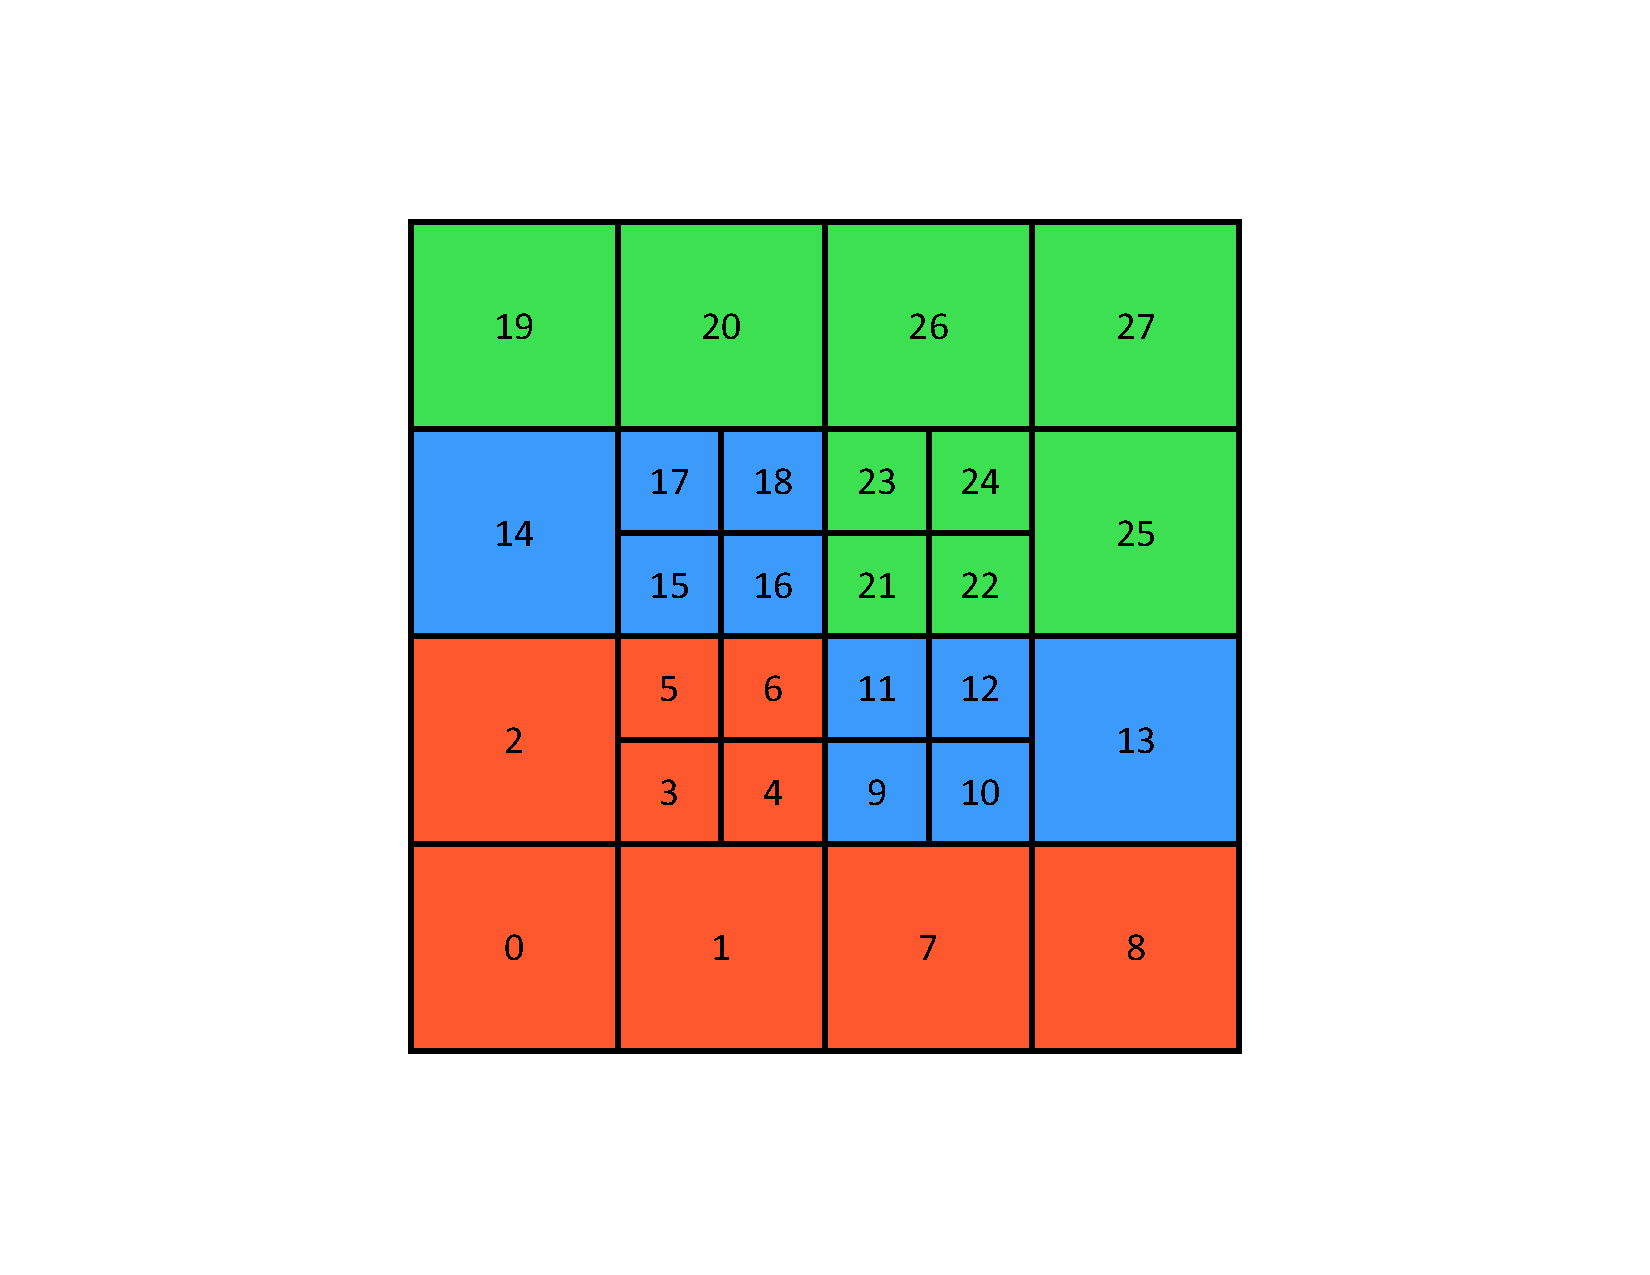
\includegraphics[width=\textwidth, clip=true, trim={0 100 0 100}]{figures/parallel_adaptive_mesh_indexing.pdf}
    \caption{An example of an adaptive, quadtree mesh that is refined around the center of the domain. The colors denote different ranks and the numbers indicate the leaf-index of the quadrant.}
    \label{fig:adaptive_mesh}
\end{figure}

\begin{figure}
    \centering
    \begin{tabular}{c}
    \smallskip
        \begin{subfigure}[t]{0.8\textwidth}
            \centering
            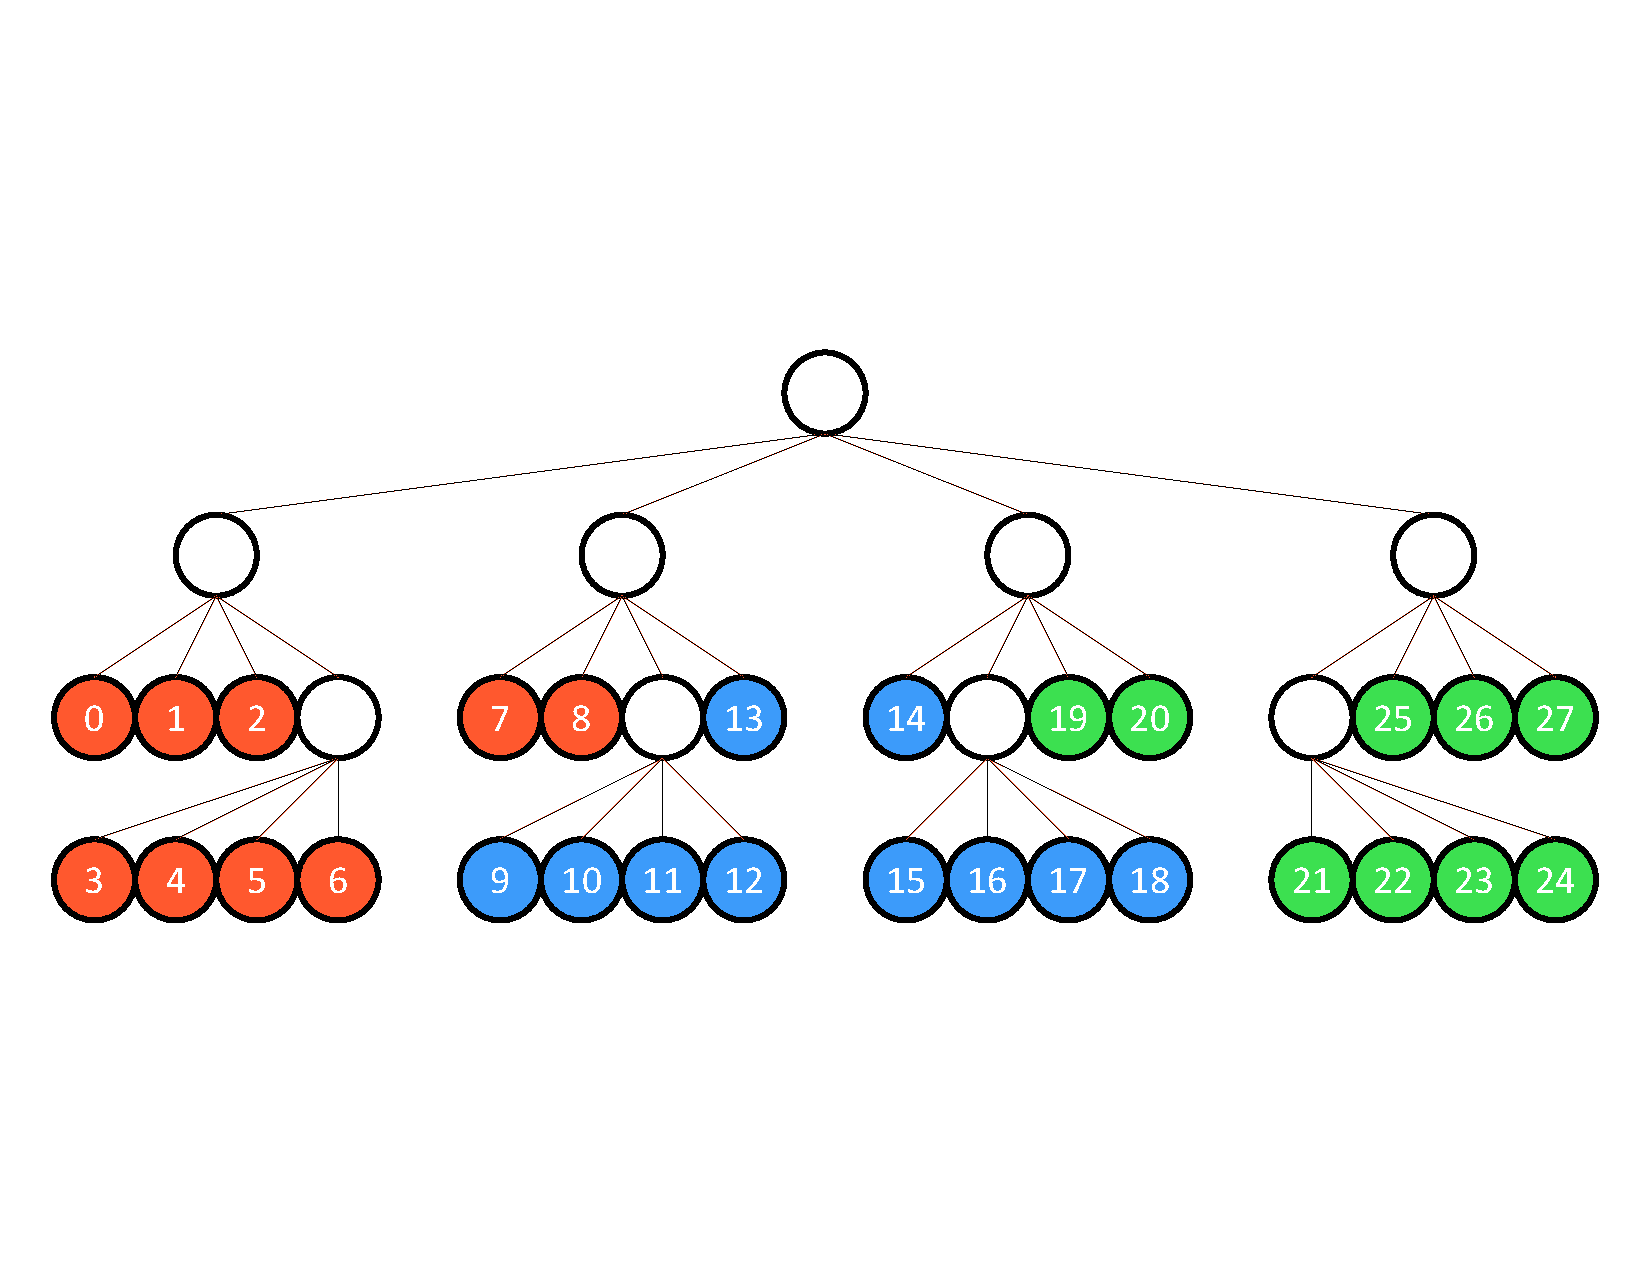
\includegraphics[width=\textwidth, clip=true, trim={0 150 0 150}]{figures/parallel_leaf_indexed_tree.pdf}
            \caption{Leaf-level indexing of quadtree nodes}
            \label{subfig:leaf-indexed-quadtree}
        \end{subfigure}
        \\
        \begin{subfigure}[t]{0.8\textwidth}
            \centering
            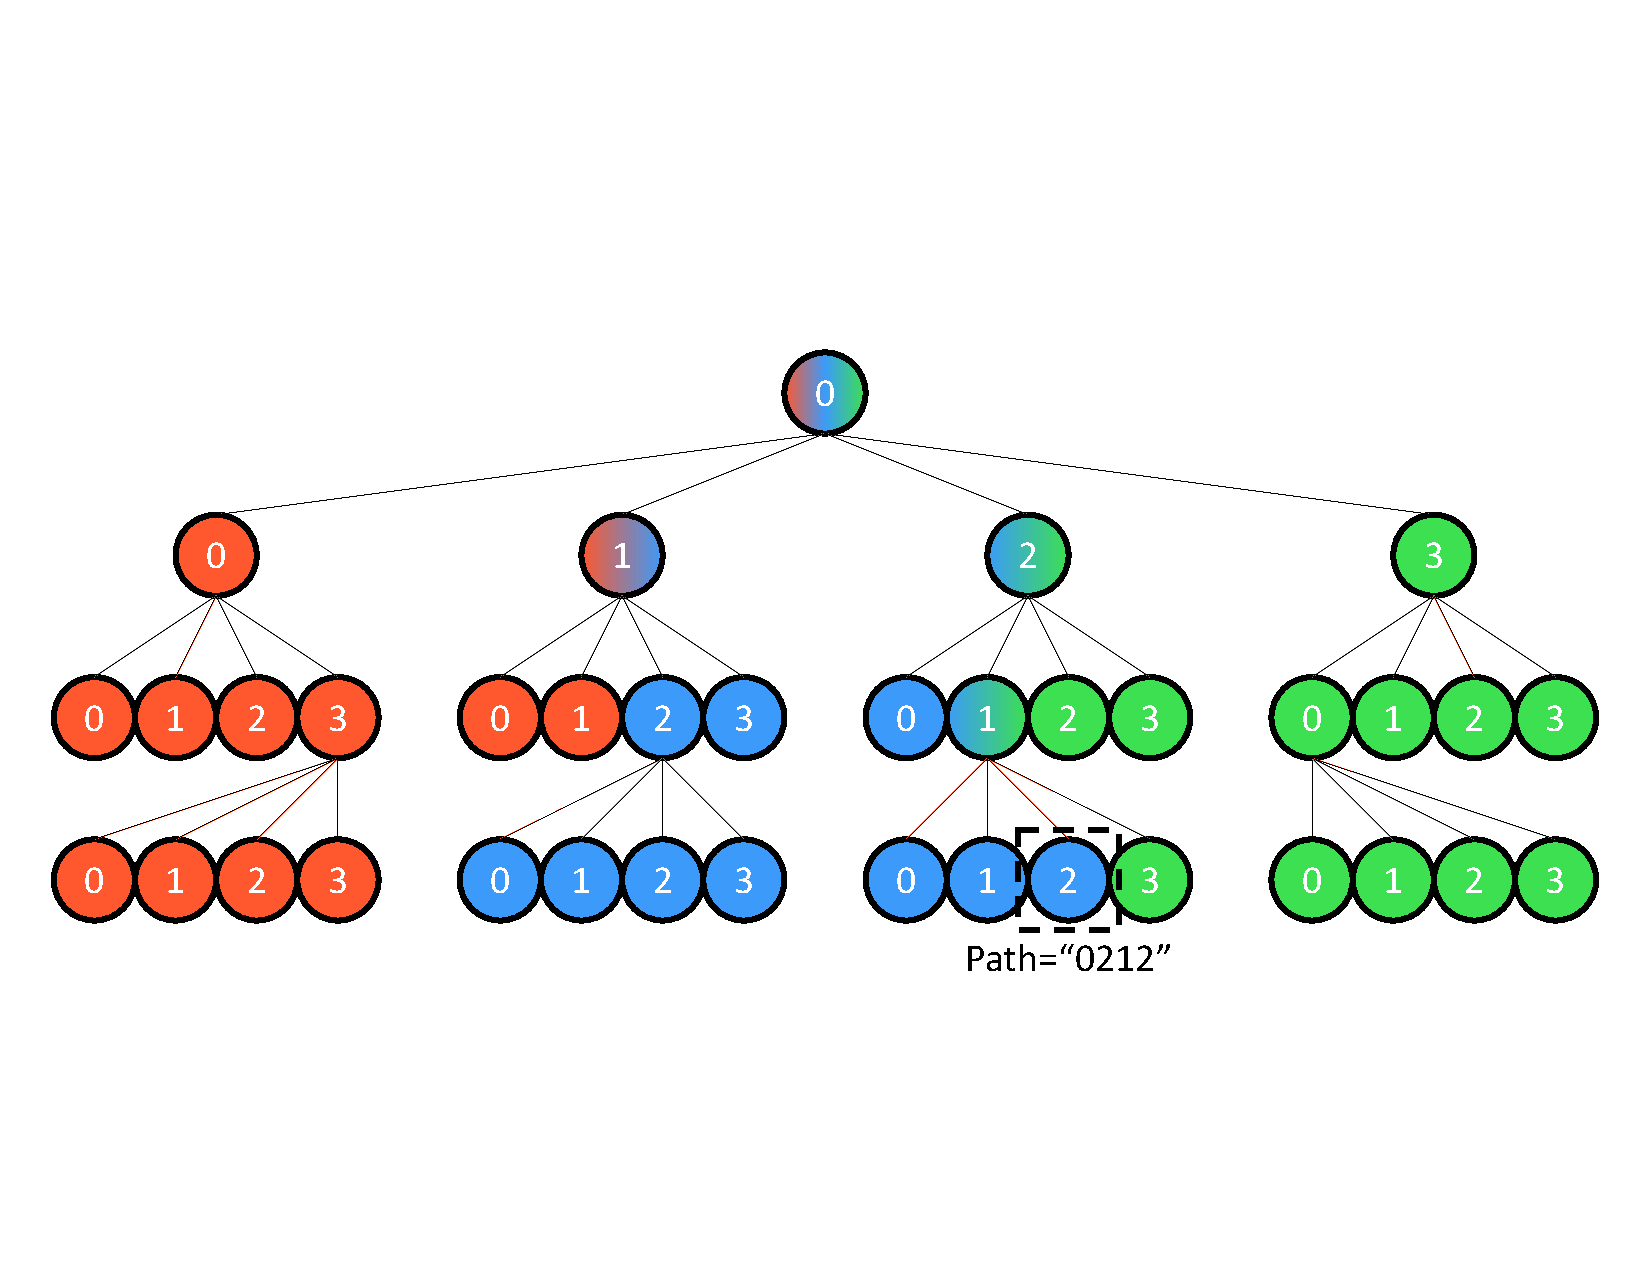
\includegraphics[width=\textwidth, clip=true, trim={0 140 0 150}]{figures/parallel_path_indexed_tree.pdf}
            \caption{Path indexing of quadtree nodes}
            \label{subfig:path-indexed-quadtree}
        \end{subfigure}
    \end{tabular}\\
    \caption{Leaf-indexed vs. path-indexed quadtrees. Both trees represent the mesh found in \reffig{fig:adaptive_mesh}. The colors denote which rank owns each node. In (a), only the leaves of a quadtree are indexed and stored. In (b), all nodes of the quadtree are indexed and stored according to their unique path. Note that the nodes in (b) that are colored with a gradient (i.e., ``0'', ``01'', ``02'', ``021'') are owned by multiple ranks.}
    \label{fig:quadtree_indexing}
\end{figure}

\subsection{Building the Set of Solution Operators}
\label{sub:building-set-of-solution-operators}

Given $\mathcal{Q}_P$, the quadtree-adaptive HPS method builds up a set of solution operators
\begin{align}
    \mathcal{S} = \{\textbf{S}^{\tau}, \textbf{w}^{\tau}\ \forall\ \tau \in \mathcal{Q}_P\}
\end{align}
such that
\begin{align}
    \textbf{u}^{\tau} = \textbf{S}^{\tau} \textbf{g}^{\tau} + \textbf{w}^{\tau},\ \forall\ \tau \in \mathcal{Q}_P.
    \label{eq:u-Sg-w}
\end{align}
The operators $\textbf{S}^{\tau}$ and $\textbf{w}^{\tau}$ are known as the solution matrix and inhomogeneous-update vector, respectively. The vector $\textbf{g}^{\tau}$ represents the provided or computed Dirichlet data for a given patch $\tau$. \refeq{eq:u-Sg-w} is used to map the known solution data on the exterior of a patch (i.e., $\textbf{g}^{\tau}$) to the interior of the patch, which is denoted by $\textbf{u}^{\tau}$.

Building up the set of solution operators $\mathcal{S}$ is the goal of the quadtree-adaptive HPS method. This is done by successively merging four children-level operators to form parent-level operators. The operators to be computed and merged are the Dirichlet-to-Neumann matrix $\textbf{T}^{\tau}$ and the inhomogeneous-flux vector $\textbf{h}^{\tau}$. Starting at the leaf-level, $\textbf{T}^{\tau}$ and $\textbf{h}^{\tau}$ are built using a {\em patch solver} function that solves \refeq{eq:elliptic-pde} on a single patch ${\Omega_i}$.

Once computed for the four children patches, the parent-level data can be computed. We denote children patches as $\alpha, \beta, \gamma,$ and $\omega$. The merged Dirichlet-to-Neumann matrix is decomposed into
\begin{align}
    \textbf{T}^{\tau} = \textbf{A} - \textbf{B} \textbf{D}^{-1} \textbf{C}
    \label{eq:T-merged}
\end{align}
where $\textbf{A}$, $\textbf{B}$, $\textbf{C}$, and $\textbf{D}$ are built from blocks of the children-level Dirichlet-to-Neumann matrices:
\begin{align}
    \textbf{A} =
    \begin{bmatrix}
        \Talphap{\tau}{\tau} & \zeromat & \zeromat & \zeromat \\
        \zeromat & \Tbetap{\tau}{\tau} & \zeromat & \zeromat  \\
        \zeromat & \zeromat & \Tgammap{\tau}{\tau} & \zeromat  \\
        \zeromat& \zeromat & \zeromat & \Tomegap{\tau}{\tau} \\
    \end{bmatrix}
    \label{eq:matrix_A}
\end{align}
\begin{align}
    \textbf{B} = 
    \begin{bmatrix}
        \Talphap{\gamma}{\tau} & \zeromat              & \Talphap{\beta}{\tau} & \zeromat \\
        \zeromat               & \Tbetap{\omega}{\tau} & \Tbetap{\alpha}{\tau} & \zeromat \\
        \Tgammap{\alpha}{\tau} & \zeromat              & \zeromat              & \Tgammap{\omega}{\tau} \\
        \zeromat               & \Tomegap{\beta}{\tau} & \zeromat              & \Tomegap{\gamma}{\tau}
    \end{bmatrix}
    \label{eq:matrix_B}
\end{align}
\begin{align}
    \textbf{C} = 
    \begin{bmatrix}
        \Talphap{\tau}{\gamma} & \zeromat               & \Tgammap{\tau}{\alpha} & \zeromat \\
        \zeromat               & \Tbetap{\tau}{\omega}  & \zeromat                & \Tomegap{\tau}{\beta} \\ 
        \Talphap{\tau}{\beta}  & \Tbetap{\tau}{\alpha} & \zeromat                & \zeromat \\
        \zeromat               & \zeromat               & \Tgammap{\tau}{\omega}  & \Tomegap{\tau}{\gamma},
    \end{bmatrix}
    \label{eq:matrix_C}
\end{align}
\begin{align}
    \textbf{D} = 
    \begin{bmatrix}
        \Talphap{\gamma}{\gamma} + \Tgammap{\alpha}{\alpha} 
        & \zeromat 
        & \Talphap{\beta}{\gamma} 
        & \Tgammap{\omega}{\alpha} \\
        % 
        \zeromat 
        & \Tbetap{\omega}{\omega} + \Tomegap{\beta}{\beta} 
        & \Tbetap{\alpha}{\omega} 
        & \Tomegap{\gamma}{\beta} \\
        % 
        \Talphap{\gamma}{\beta} 
        & \Tbetap{\omega}{\alpha} 
        & \Talphap{\beta}{\beta}+ \Tbetap{\alpha}{\alpha} 
        & \zeromat \\
        % 
        \Tgammap{\alpha}{\omega} 
        & \Tomegap{\beta}{\gamma} 
        & \zeromat 
        & \Tgammap{\omega}{\omega} + \Tomegap{\gamma}{\gamma}
    \end{bmatrix}
    \label{eq:matrix_D}.
\end{align}
The subscripts of each Dirichlet-to-Neumann matrix $\textbf{T}^{k}_{ij}$ indicate a mapping from Dirichlet data from the edge $i$ to Neumann data on edge $j$ of patch $k$.

The merged inhomogeneous-flux vector $\textbf{h}^{\tau}$ is computed as
\begin{align}
    \textbf{h}^{\tau} = -\textbf{h}_{\text{ext}} + \textbf{B} \textbf{D}^{-1} \Delta \textbf{h}
    \label{eq:h-merged}
\end{align}
where $\textbf{h}_{\text{ext}}$ corresponds to the exterior of $\Omega_{\tau}$ and
\begin{align}
    \Deltah = 
    \begin{bmatrix}
        \halphap{\gamma} + \hgammap{\alpha} \\
        \hbetap{\omega} + \homegap{\beta} \\
        \halphap{\beta} + \hbetap{\alpha} \\
        \hgammap{\omega} + \homegap{\gamma}
    \end{bmatrix}.
    \label{eq:delta_h}
\end{align}

The merged, parent-level solution matrix and inhomogeneous-update vector are computed from children-level patches as
\begin{align}
    \textbf{S}^{\tau} &= -\textbf{D}^{-1} \textbf{C}
    \label{eq:S-merged} \\
    \textbf{w}^{\tau} &= -\textbf{D}^{-1} \Deltah.
    \label{eq:w-merged}
\end{align}

\subsection{Stages of the Quadtree-Adaptive HPS Method}
\label{sub:stages-of-the-quadtree-adaptive-hps-method}

Algorithmically, the quadtree-adaptive HPS method is implemented with three stages: a build stage, an upwards stage, and a solve stage. The build stage computes $\textbf{T}^{\tau}$ and $\textbf{S}^{\tau}\ \forall\ \tau \in \mathcal{Q}_P$. The upwards stage computes $\textbf{h}^{\tau}$ and $\textbf{w}^{\tau}\ \forall\ \tau \in \mathcal{Q}_P$. Building up the set of solution operators $\mathcal{S}$ is split into the build and the upwards stage to reduce redundant calculations when solving \refeq{eq:elliptic-pde} with a homogeneous RHS, or $f(\textbf{x}) = 0$. The solve stage applies the solution operators $\textbf{S}^{\tau}$ and $\textbf{w}^{\tau}$ from the set $\mathcal{S}$ to supplied  Dirichlet boundary data $\textbf{g}^{\tau}$ on $\Omega_D$  according to \refeq{eq:u-Sg-w}.

In each of the stages, there are two traversals of the quadtree $\mathcal{Q}_P$: a leaf traversal and a family traversal. A leaf traversal visits each of the leaf nodes in the leaf-indexed or path-indexed quadtree (the leaf nodes for both trees are identical). A family traversal visits each family of the quadtree, where a family consists of four children nodes and a parent node. Family traversals can be done in a pre-order fashion (start at the root and visit families before moving down the tree) or in a post-order fashion (start at the leaf nodes and visit families before moving up the tree). Details on how to traverse a leaf- or path-indexed quadtree will be provided in \refsec{sub:quadtree-data-structures}.

\subsubsection{The Build Stage}

The leaf traversal of the build stage computes $\textbf{T}^{\tau}$ for all leaf-level patches. As outlined in \citep{chipman2024fast}, this is done by calling a patch solver that employs fast methods to solve \refeq{eq:elliptic-pde}. \refeq{eq:elliptic-pde} is solved with unit potentials placed on each of the cell centers on the boundary of the leaf-level patch to compute the columns of $\textbf{T}^{\tau}$.

The family traversal of the build stage is outlined in \refalg{alg:build_merge} and is done in a post-order fashion. The goal of the 4-to-1 merge is to compute the parent-level Dirichlet-to-Neumann matrix and the solution operator from the four children patches. This is done with \refeq{eq:T-merged} and \refeq{eq:S-merged}.

\begin{algorithm}
    \caption{\texttt{Merge4To1} Function (Build Stage Family Callback)}
    \begin{algorithmic}[0]
        \Require $\textbf{T}^{\alpha}$, $\textbf{T}^{\beta}$, $\textbf{T}^{\gamma}$, $\textbf{T}^{\omega}$
        \For{$i = \alpha, \beta, \gamma, \omega$}
            \State \texttt{tag} = \texttt{TagForCoarsening}(i)
            \If{\texttt{tag}}
                \State Coarsen: $\textbf{T}^{i} = \textbf{L}_{2,1} \textbf{T}^{i} \textbf{L}_{1,2}$
            \EndIf
        \EndFor
        \State Compute matrices $\textbf{A}, \textbf{B}, \textbf{C}, \textbf{D}$ according to \refeq{eq:matrix_A} - \refeq{eq:matrix_D}. 
        \State Compute $\textbf{S}^{\tau} = \textbf{D}^{-1} \textbf{C}$
        \State Compute $\textbf{T}^{\tau} = \textbf{A} - \textbf{B} \textbf{D}^{-1} \textbf{C}$
    \end{algorithmic}
    \label{alg:build_merge}
\end{algorithm}

\subsubsection{The Upwards Stage}

The leaf traversal of the upwards stage computes $\textbf{h}^{\tau}$ for all leaf-level patches. The is done by calling the same routine used to build $\textbf{T}^{\tau}$ on leaf-level patches in the build stage, while supplying zero Dirichlet boundary conditions: $\textbf{g}^{\tau} = \textbf{0}$.

The family traversal is outlined in \refalg{alg:upwards_merge} and is also done in a post-order fashion. The upwards 4-to-1 merge computes the merged inhomogeneous-flux vector $\textbf{h}^{\tau}$ via \refeq{eq:h-merged} and the inhomogeneous-update vector $\textbf{w}^{\tau}$ via \refeq{eq:w-merged}.

\begin{algorithm}
    \caption{\texttt{Upwards4To1} Function (Upwards Stage Family Callback)}
    \begin{algorithmic}[0]
        \Require $\textbf{T}^{\alpha}$, $\textbf{T}^{\beta}$, $\textbf{T}^{\gamma}$, $\textbf{T}^{\omega}$, $\textbf{h}^{\alpha}$, $\textbf{h}^{\beta}$, $\textbf{h}^{\gamma}$, $\textbf{h}^{\omega}$
        \For{$i = \alpha, \beta, \gamma, \omega$}
        \State \texttt{tag} = \texttt{TagForCoarsening}(i)
        \If{\texttt{tag}}
        \State Coarsen: $\textbf{h}^{i} = \textbf{L}_{2,1} \textbf{h}^{i}$
        \EndIf
        \EndFor
        \State Compute matrices $\textbf{B}, \textbf{D}$ according to \refeq{eq:matrix_B} and \refeq{eq:matrix_D}
        \State Compute $\Delta \textbf{h}$ according to \refeq{eq:delta_h}
        \State Compute $\textbf{h}^{\tau} = \textbf{h}^{\tau} + \textbf{B} \textbf{w}^{\tau}$
        \State Compute $\textbf{w}^{\tau} = -\textbf{D}^{-1} \Deltah$.
    \end{algorithmic}
    \label{alg:upwards_merge}
\end{algorithm}

\subsubsection{The Solve Stage}

The goal of the solve stage is to apply the now computed solution matrix $\textbf{S}^{\tau}$ and inhomogeneous-update vector $\textbf{w}^{\tau}$ to provided Dirichlet data at the root down the tree until all leaf-level nodes have Dirichlet data. This constitutes the family traversal (found in \refalg{alg:solve_split}) that is done in a pre-order fashion.

The leaf traversal is then a final step to iterate over all the leaf-level patches and solve \refeq{eq:elliptic-pde} on the subdomains using fast methods. This is an independent step for each leaf-level patch and can be done simultaneously everywhere, taking advantage of the domain decomposition.

\begin{algorithm}
    \caption{\texttt{Split1To4} Function (Solve Stage Family Callback)}
    \begin{algorithmic}[0]
        \Require $\textbf{S}^{\tau}$, $\textbf{g}^{\tau} = \textbf{u}^{\tau}_{ext}$
        \State \texttt{tag} = \texttt{TagForUncoarsening}($\tau$)
        \If{\texttt{tag}}
            \State Uncoarsen: $\textbf{g}^{\tau} = \textbf{L}_{1,2} \textbf{g}^{\tau}$
        \EndIf
        \State Compute $\textbf{u}^{\tau}_{\text{int}} = \textbf{S}^{\tau} \textbf{g}^{\tau} + \textbf{w}^{\tau}$
        \State Partition $\textbf{u}^{\tau}_{\text{int}}$ into $\textbf{u}^{\alpha}_{\text{ext}}, \textbf{u}^{\beta}_{\text{ext}}, \textbf{u}^{\gamma}_{\text{ext}}, \textbf{u}^{\omega}_{\text{ext}}$
    \end{algorithmic}
    \label{alg:solve_split}
\end{algorithm}